\let\negmedspace\undefined
\let\negthickspace\undefined
\documentclass[journal]{IEEEtran}
\usepackage[a5paper, margin=10mm, onecolumn]{geometry}
%\usepackage{lmodern} 
\usepackage{tfrupee} 

\setlength{\headheight}{1cm} 
\setlength{\headsep}{0mm}     

\usepackage{gvv-book}
\usepackage{gvv}
\usepackage{cite}
\usepackage{amsmath,amssymb,amsfonts,amsthm}
\usepackage{algorithmic}
\usepackage{graphicx}
\usepackage{textcomp}
\usepackage{xcolor}
\usepackage{txfonts}
\usepackage{listings}
\usepackage{enumitem}
\usepackage{mathtools}
\usepackage{gensymb}
\usepackage{comment}
\usepackage[breaklinks=true]{hyperref}
\usepackage{tkz-euclide} 
\usepackage{listings}                                        
\def\inputGnumericTable{}                                 
\usepackage[latin1]{inputenc}                                
\usepackage{color}                                            
\usepackage{array}                                            
\usepackage{longtable}                                       
\usepackage{calc}                                             
\usepackage{multirow}                                         
\usepackage{hhline}                                           
\usepackage{ifthen}                                           
\usepackage{lscape}

\begin{document}

\bibliographystyle{IEEEtran}
\vspace{3cm}

\title{2.6.9}
\author{AI25BTECH11003 - Bhavesh Gaikwad}
{\let\newpage\relax\maketitle}

\renewcommand{\thefigure}{\theenumi}
\renewcommand{\thetable}{\theenumi}
\setlength{\intextsep}{10pt} 


\numberwithin{equation}{enumi}
\numberwithin{figure}{enumi}
\renewcommand{\thetable}{\theenumi}


\textbf{Question}: The area of a triangle with vertices A(3,0), B(7,0) and C(8,4) is\\\\

\textbf{Solution:}\\
Given: $A(3,0),\; B(7,0),\; C(8,4).$\\

$
\vec{B}-\vec{A}=\myvec{7-3\\0-0}
=\myvec{4\\0},\qquad
\vec{C}-\vec{A}=\myvec{8-3\\4-0} = \myvec{5\\4}.
$\\

$\norm{\vec{(B-A)} \times \vec{(C-A)}} = \norm{\,\myvec{|\vec{A_{23}} & \vec{B_{23}}| \\ |\vec{A_{31}} & \vec{B_{31}}| \\ |\vec{A_{12}} & \vec{B_{12}}|}\,} = 16 $\\\\


$
\text{Area}=\frac{1}{2}\norm{\vec{(B-A)} \times \vec{(C-A)}} = 8
$

\begin{align}
    \centering
    \boxed{Area \, of \, Triangle \, ABC \,= \,8\,sq.units}
\end{align}
\bigskip

\begin{figure}[htbp]
    \centering
    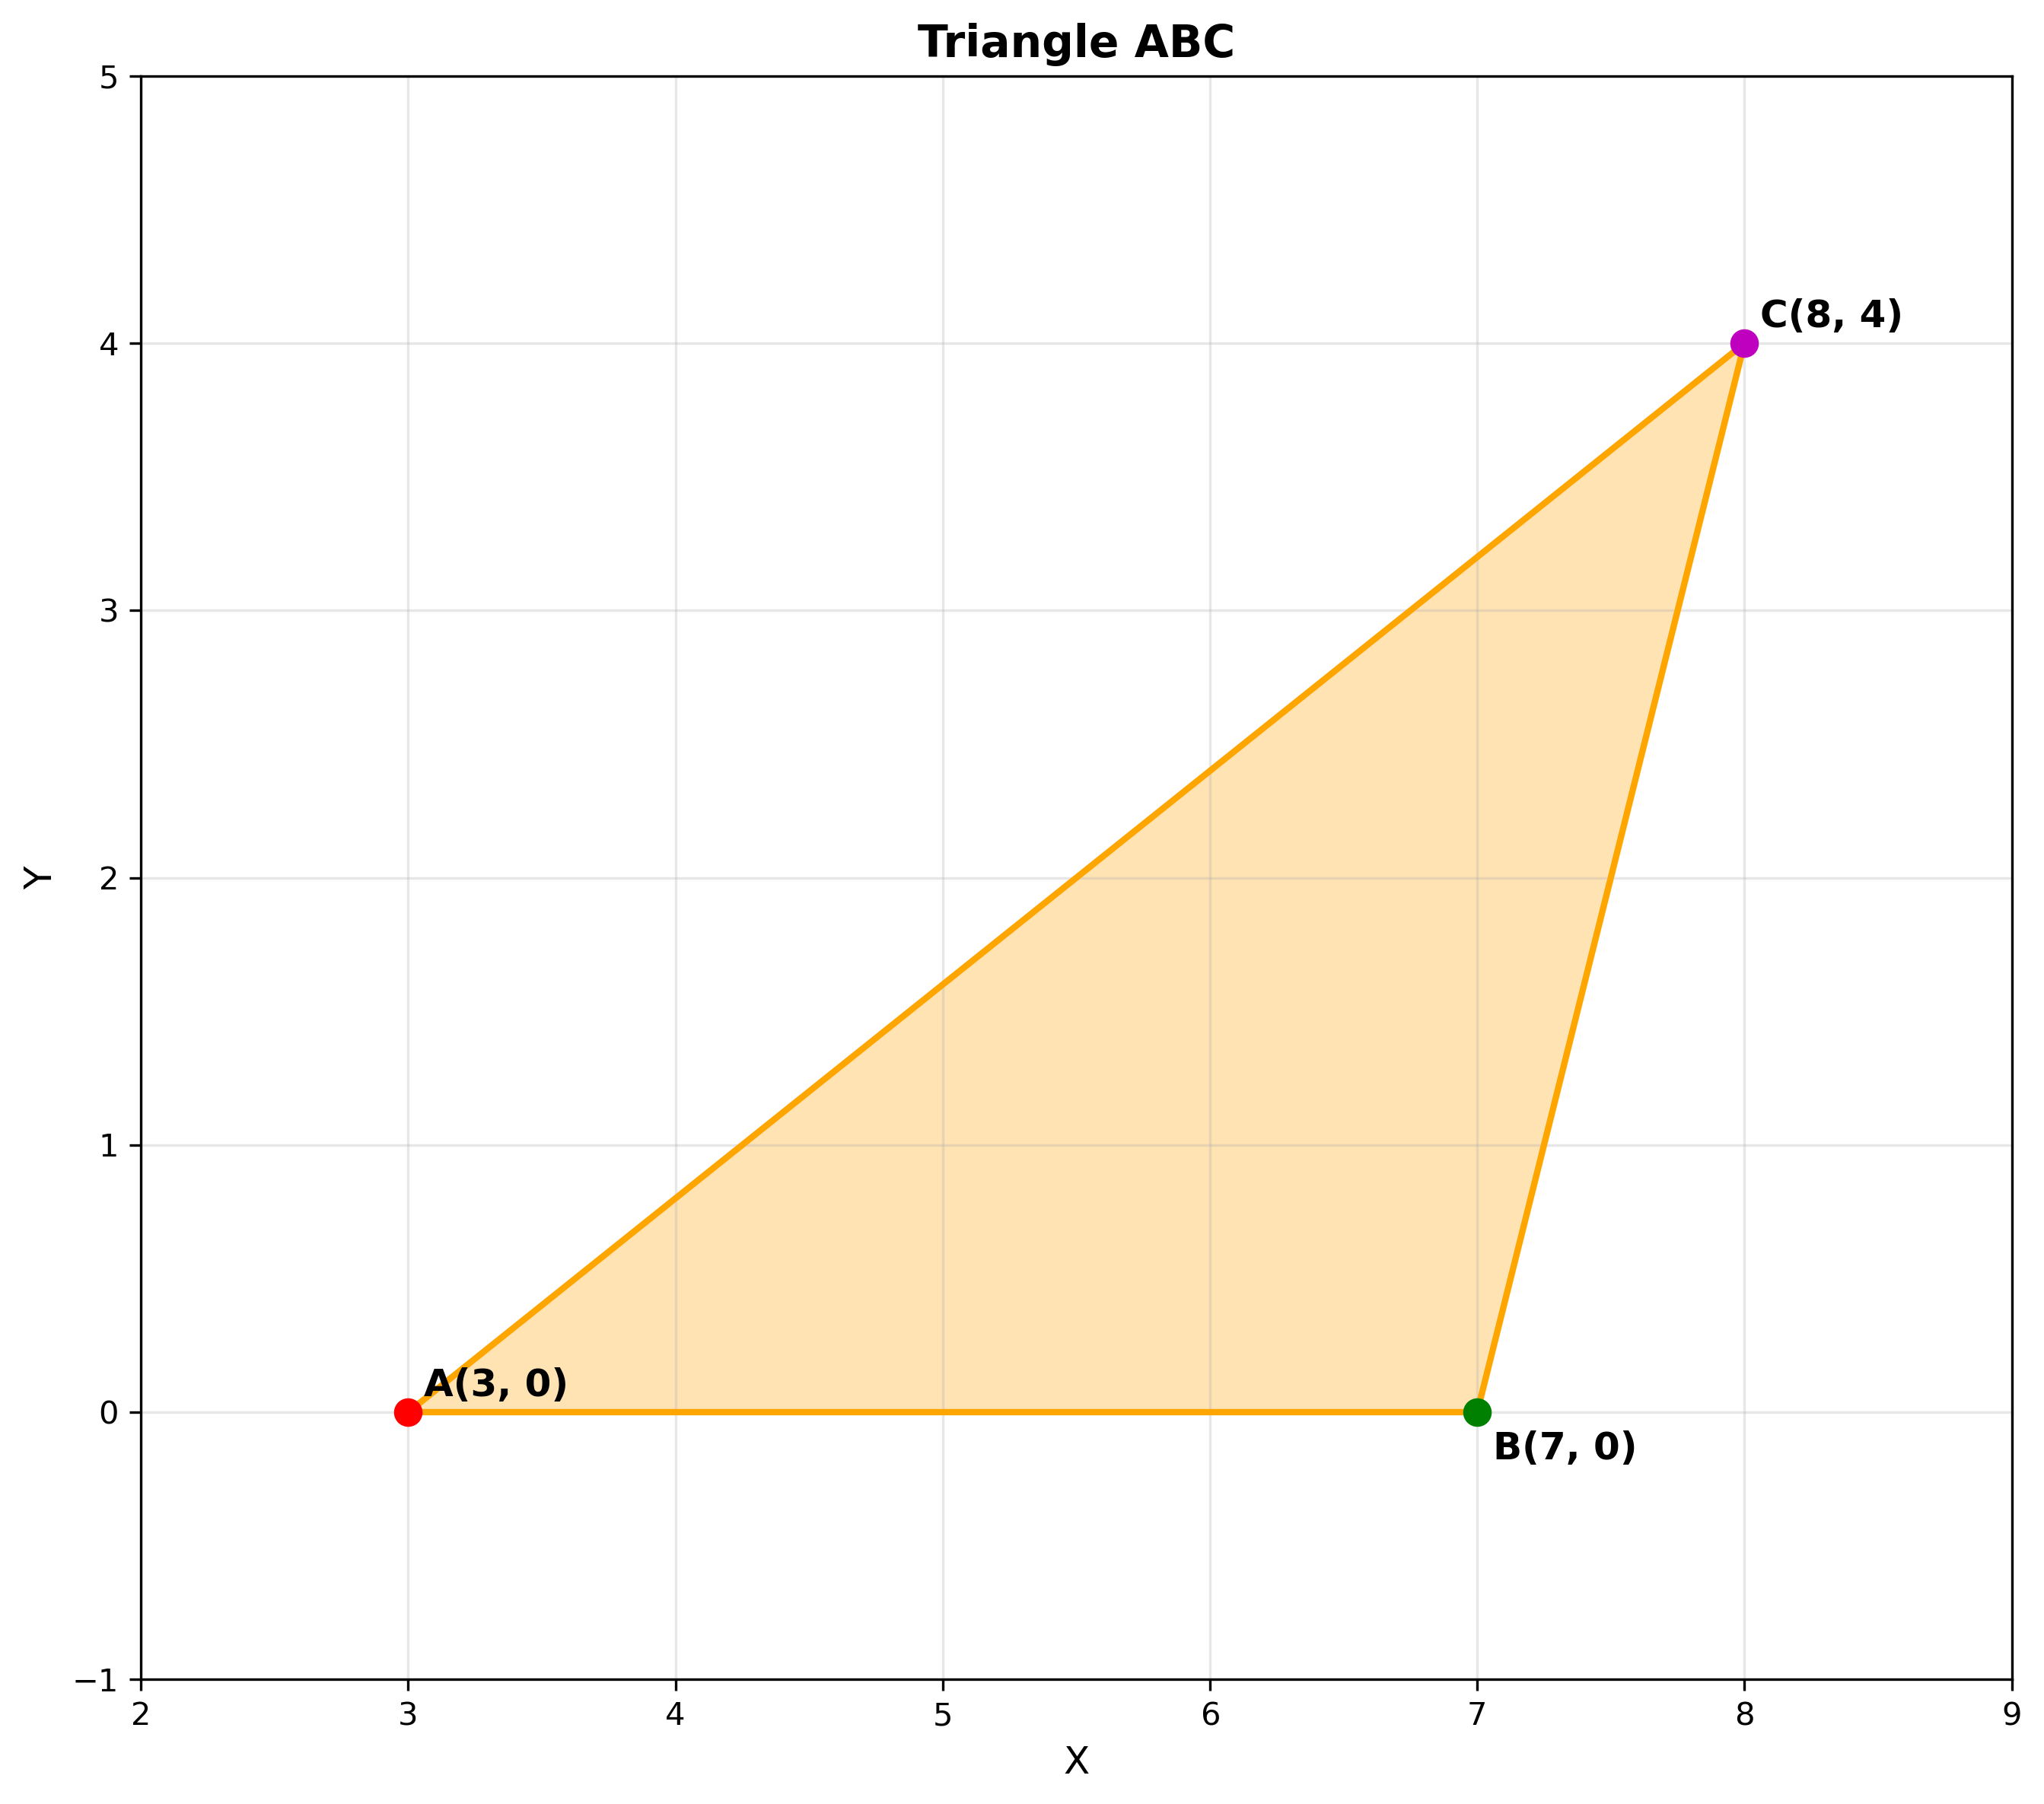
\includegraphics[width=0.65\linewidth]{figs/fig1.png}
    \caption{Vector Representation}
    \label{fig:fig/fig1.png}
\end{figure}
\end{document}  
